\section{Introduction}

\begin{frame}{Background}
\begin{figure}
    \centering
    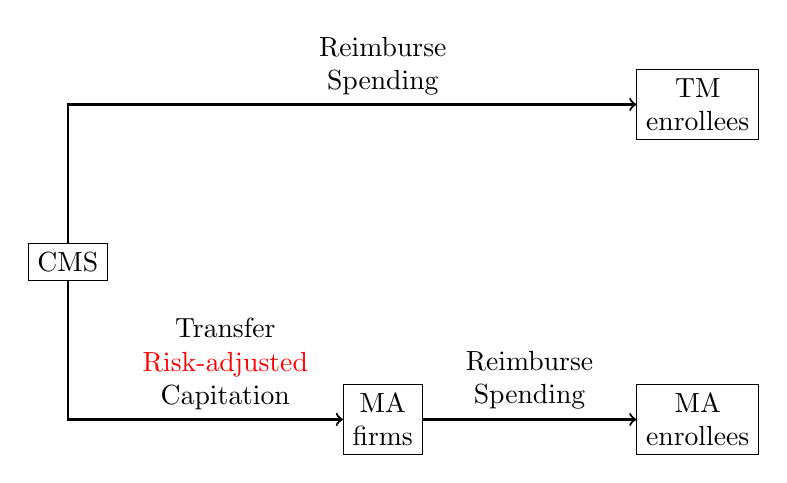
\begin{tikzpicture}
    \node[draw] (CMS) at (0,2) {CMS};
    \node[draw, align=center] (TM) at (8,4) {TM \\ enrollees};
    \node[draw, align=center] (MA) at (8,0) {MA \\ enrollees};
    \node[draw, align=center] (MAf) at (4,0) {MA \\ firms};

    \draw[->, thick] (CMS.north) |- (TM.west);
    \draw[->, thick] (CMS.south) |- (MAf.west);
    \draw[->, thick] (MAf.east) -- (MA.west) node[midway, above, align=center] {Reimburse \\ Spending};

    \node[above, align=center] at (4,4) {Reimburse \\ Spending};
    \node[above, align=center] at (2,0) {Transfer \\ \textcolor{red}{Risk-adjusted} \\ Capitation};
\end{tikzpicture}
    \caption{Medicare Market Structure}
\end{figure}
\end{frame}

\begin{frame}{Illustrative Distribution Example}
    \framesubtitle{What if No Risk Adjustment}
    \begin{figure}
        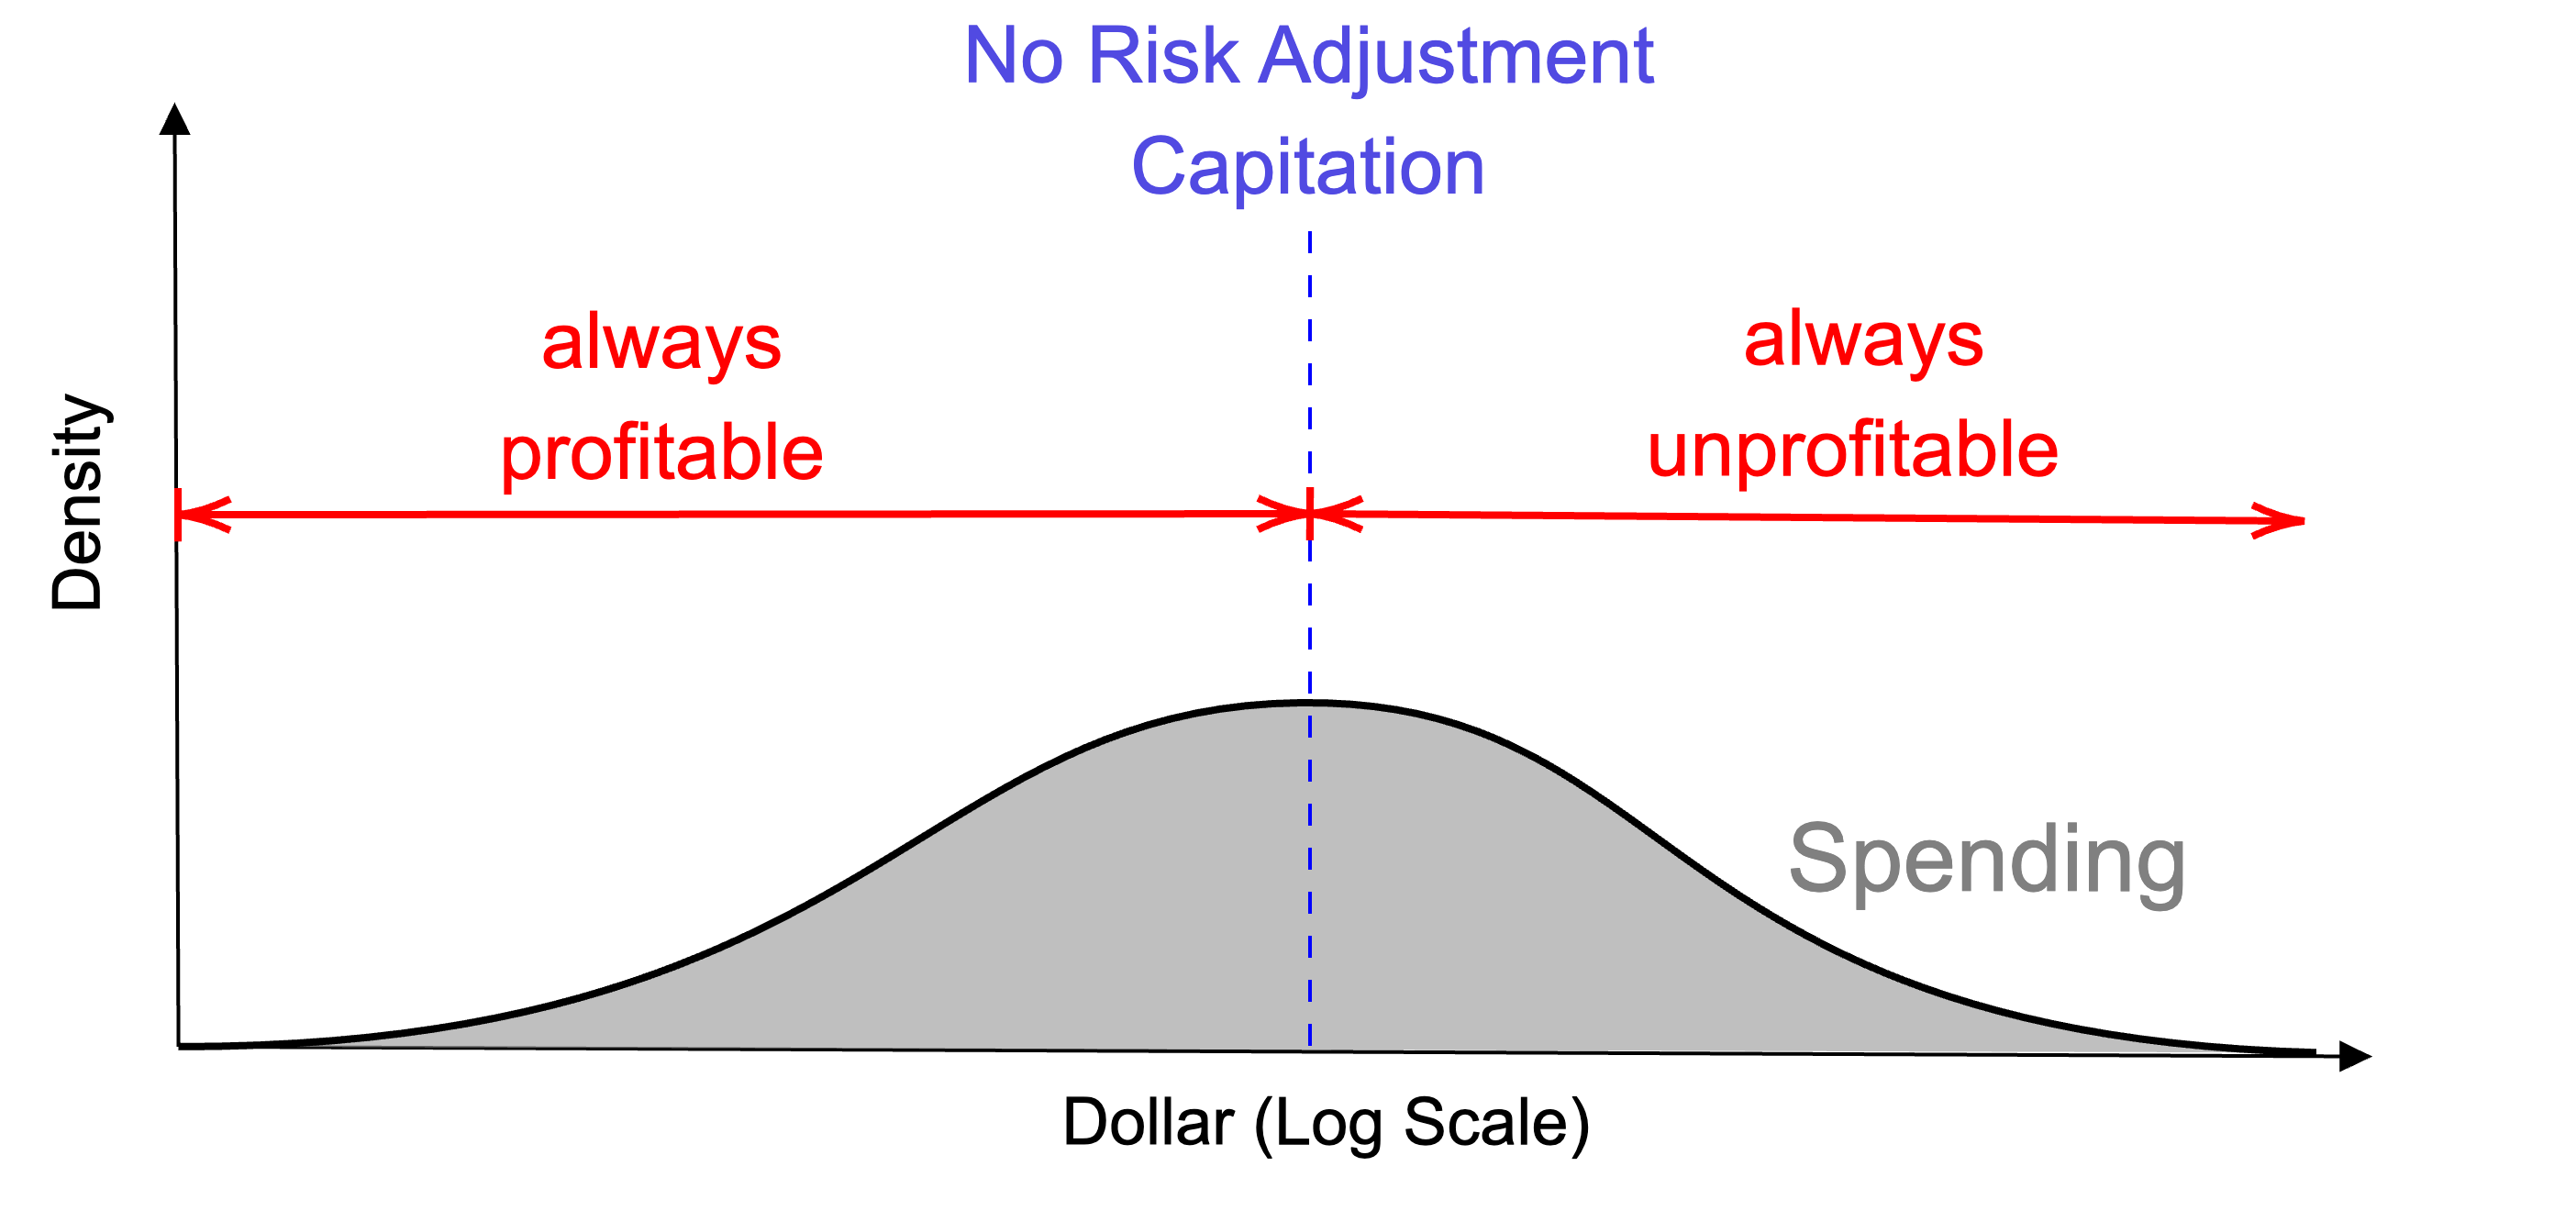
\includegraphics[width=0.8\textwidth]{figures/images/example_0.png}
        \caption{Example Distribution of Capitation and Spending}
    \end{figure}
\end{frame}


\begin{frame}[label=example_distribution]{Illustrative Distribution Example}
    \framesubtitle{What if Imperfect Risk Adjustment}
    \begin{figure}
        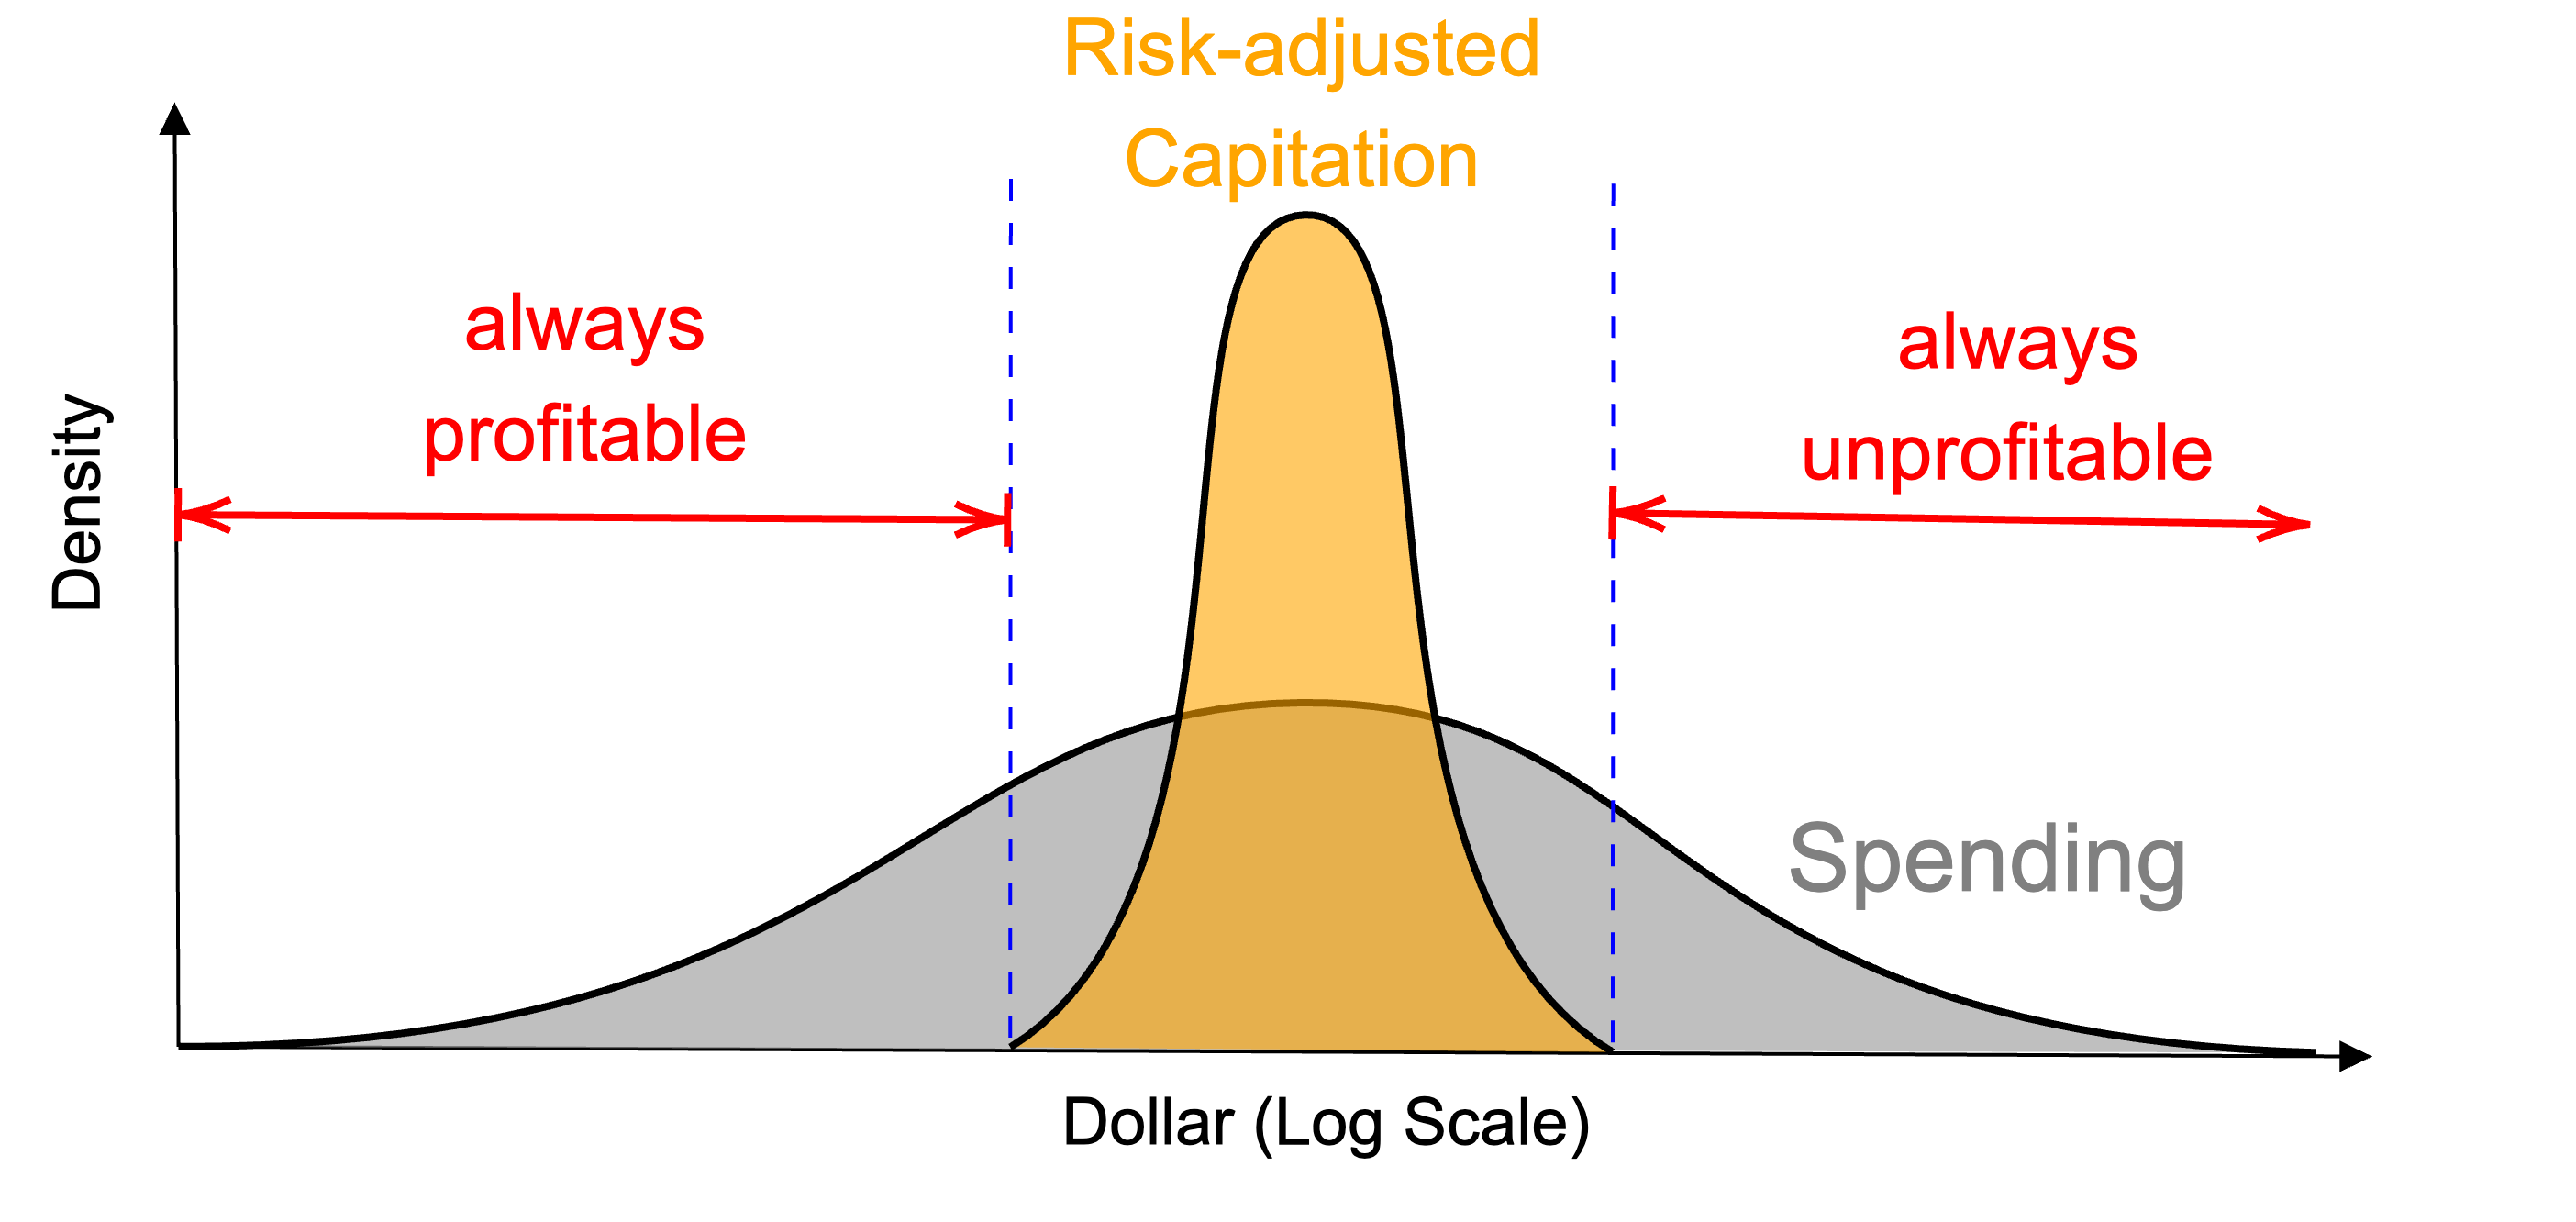
\includegraphics[width=0.8\textwidth]{figures/images/example_1.png}
        \caption{Example Distribution of Capitation and Spending}
    \end{figure}
    \hyperlink{actual_distribution}{\beamergotobutton{Actal Distribution}}
    \hyperlink{example_alternative}{\beamergotobutton{Example Aternative}}
\end{frame}


\begin{frame}{Selection Incentive}
    \framesubtitle{Under Imperfect Risk Adjustment}
    \textbf{Observation:} Regardless of their capitation rates:
    \begin{itemize}
        \item Consumers on the far left (very low spending) are always profitable.
        \item Consumers on the far right (very high spending) always induce huge losses.
        \item Profitability differences drive selection motives.
    \end{itemize}
    
    \vfill 

    \textbf{If:} 
    \begin{itemize}
        \item \textcolor{structure}{Actual distritution is similar to (Imperfect Risk Adjustment) example.} 
    \end{itemize}

    \textbf{Then MA firms have:} 
    \begin{itemize}
        \item  incentive to attract the healthy. 
    \end{itemize}
\end{frame}

\begin{frame}{Story: (Implicit) Selection via Plan Design}
    With the selection incentive

    \textbf{If:} 
    \begin{itemize}
        \item \textcolor{structure}{A generous outside option is always available.}
        \item \textcolor{structure}{Consumers' health perceptions provide extra insight into spending.}
        \item \textcolor{structure}{Health perceptions influence individual preferences for generosity.}
    \end{itemize}
    
    \textbf{Then MA firms can:} 
    \begin{itemize}
        \item  design \textit{cheap} low generosity plans $\rightarrow$ attract ``healthy'' $\rightarrow$ maximize profit.
    \end{itemize}

    \vfill
    \pause
    \textbf{Implication:}
    \begin{itemize}
        \item Current Risk Adjustment falls short in eliminating selection incentives.
    \end{itemize}
    \renewcommand*{\thefootnote}{}
    \footnotetext{Note: By law, MA firms cannot explicitly select or discrimate consumers.}
\end{frame}


\begin{frame}{Research Questions}
    \begin{itemize}
        \item How does risk adjustment influence selection incentives and consequently affect the plan design of MA firms?
        

        \item What are the welfare implications of the aforementioned behaviors?

    \end{itemize}
\end{frame}